In order to compute optimal paths that include also sharing vehicles, not included into the set of possible travel means offered by \textit{Google Map APIs}, the system will have to implement some additional logic. We will handle the sharing vehicles option as an additional possible public travel mean, for example an user could want to take a bike in sharing instead of taking the subway.\\
The algorithm that implement this functionality will follow the behavior explained in the pseudo-code below:
\begin{figure}[H]
\begin{center}
		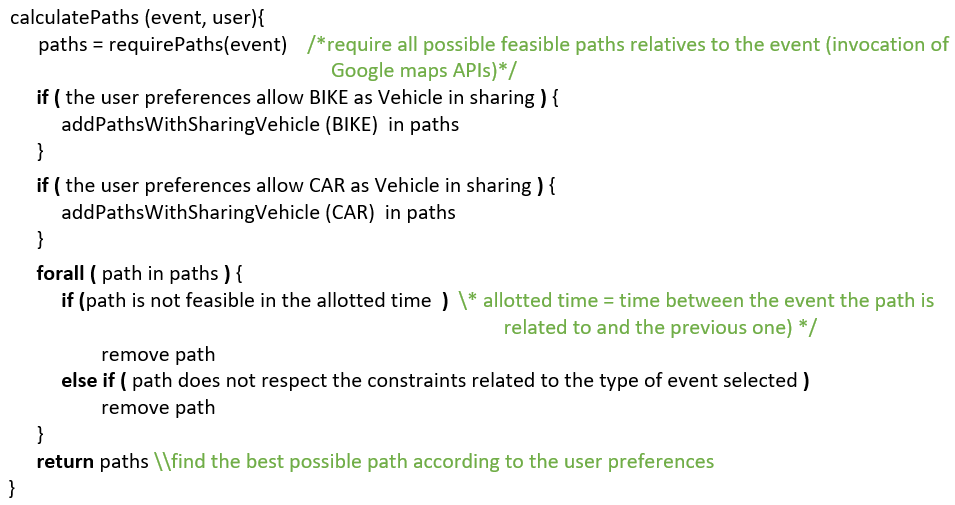
\includegraphics[width=\textwidth]{algorithms/calculate_paths.png}
\end{center}
\end{figure}
\noindent The addPathsWithSharingVehicle method is explained below:
\begin{figure}[H]
\begin{center}
		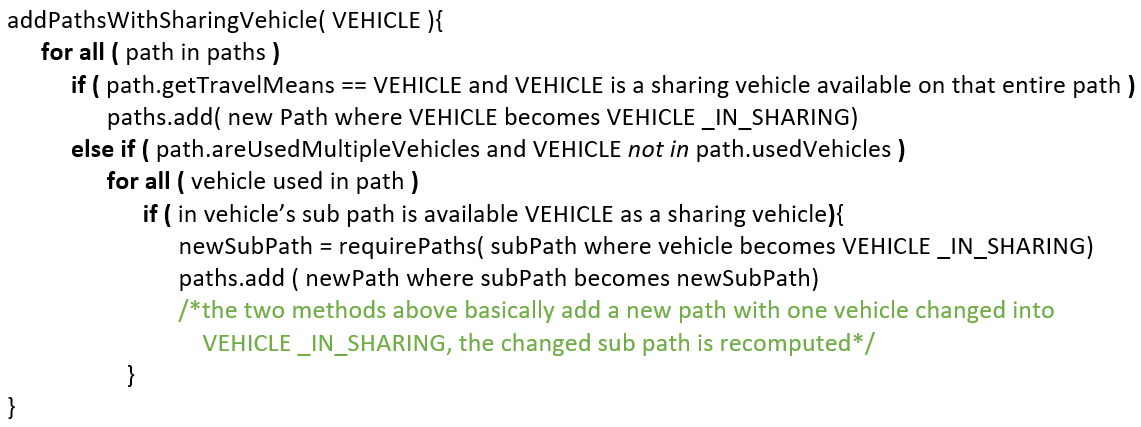
\includegraphics[width=\textwidth]{algorithms/sharing_method.png}
		
\end{center}
\end{figure}
